\documentclass[11pt,compress,mathserif]{beamer}
\usepackage{latexsym,amsmath,amssymb,amsfonts}
\usepackage{graphicx,subfigure, color,epsfig,fancyhdr}
\usepackage{mathrsfs,bbm,dsfont}
\usepackage{algorithm}
\usepackage{algorithmic}
\usepackage{algpseudocode}
\usepackage{multirow}
\hypersetup{pdfpagemode=FullScreen}
\usepackage{multimedia}
\usepackage{beamerthemesplit}
\usetheme{Copenhagen}
\usecolortheme[rgb={0.2,0.2,0.5}]{structure}%0-1.
\setbeamercolor{alerted text}{fg=violet}
\newenvironment{eqn}{\begin{equation}}{\end{equation}}
\newenvironment{eqar}{\begin{eqnarray}}{\end{eqnarray}}
\newenvironment{eqar*}{\begin{eqnarray*}}{\end{eqnarray*}}
\newenvironment{enumerate-roman}{\begin{enumerate}\renewcommand{\labelenumi}{(\roman{enumi})}}{\end{enumerate}}
\newenvironment{enumerate-Roman}{\begin{enumerate}\renewcommand{\labelenumi}{\Roman{enumi}.}}{\end{enumerate}}
\newenvironment{prf}[1][Proof]{\noindent\textbf{#1.} }{\hfill$\square$}
\newcommand{\pf}{\hfill$\square$}
\newcommand{\oiint}{\mathop{\makebox[-0.32em][l]{$\bigcirc$}\int\!\!\!\!\!\int\makebox[-0.5em]{}}}
\newcommand{\tr}{\mbox{tr}}
\newtheorem{thm}{Theorem}[section]
\newtheorem{prop}[thm]{Proposition}
\newtheorem{prope}[thm]{Properties}
\newtheorem{lem}[thm]{Lemma}
\newtheorem{defn}[thm]{Definition}
\newtheorem{cor}[thm]{Corollary}
\newtheorem{rem}[thm]{Remark}
\newtheorem{eg}[thm]{Example}
\newtheorem{thm2}{Theorem*}
%\newtheorem{}[thm]{}

\frenchspacing
\allowdisplaybreaks

\expandafter\def\expandafter\insertshorttitle\expandafter{%
	\insertshorttitle\hfill%
	\insertframenumber\,/\,\inserttotalframenumber}

%============================================================

\begin{document}

\title[xxx]{Simulated Quantum Annealing xxx}

\author[xxx]{xxx } 
\date{\footnotesize Group Project Presentation \\ \today \\
\vspace{0.4cm}
\emph{Supervisor: Dr. RUIZ Matias}}

%============================================================

\frame{\titlepage}

%============================================================

% \section[$\bigstar$]{}%Time: 0.5 min
\frame{\begin{small}\tableofcontents\end{small}}

%============================================================

\section[Intro]{Introduction}

\begin{frame}\frametitle{Introduction}
\bit
\item Simulated Quantum Annealing (SQA) relates certain quantum systems to classical Markov chains.
% is a Markov Chain Monte-Carlo algorithm that samples the equilibrium thermal state of a Quantum Annealing (QA) Hamiltonian.

\item One piece of evidence for the strength of QA over classical simulated annealing comes from an example by Farhi, Goldstone and Gutmann.

\item Crosson and Harrow showed that the Markov chain underlying SQA can efficiently sample the target distribution and find the global minimum of this spike cost function in polynomial time. 

\item SQA inherits at least some of the advantages of tunneling in QA, and so QA is unlikely to achieve exponential speedups over classical computing solely by the use of quantum tunneling. 
\eit
\end{frame}

%============================================================

% \subsection[Review]{Literature Review}
% \begin{frame}\frametitle{Literature Review}

% \textcolor{blue}{paper: 'Simulated Quantum Annealing Can Be Exponentially Faster than Classical Simulated Annealing'\\
% 'Quantum Adiabatic Evolution Algorithms versus Simulated Annealing'}

% \end{frame}

%============================================================

\section[SA]{Simulated Annealing}

\begin{frame}\frametitle{Simulated Annealing (SA)}

\bit

\item A classical local search strategy to find the global minimum of a cost function $h(z_1, \cdots, z_n)$.
% can be viewed as taking a random walk in the problem space according to a Markov chain parameterized by temperature

\item Construct a Markov chain starts in the $\gamma = \infty$ Boltzmann distribution and gradually moves through the Boltzmann distributions for decreasing $\gamma$ down to $\gamma$ near 0.
% If the process succeeds, the final distribution will be close to the zero temperature Boltzmann distribution, which means that the global minimum of h has been found with high probability.

\item Follows the Metropolis rule \cite{metropolis1953equation}, the probability is
\begin{align}
    \label{eq1}
    P\left(z, z^{\prime}\right)=\min \left\{1, \exp \left(-\Delta h / T\right)\right\}  
\end{align}
for an attempted spin flip $z \rightarrow z^{\prime}$.
% which is the probability that a spin flip is allowed
% the rules guarantees that if many transitions are made at a single temperature T, the distribution of the string will converge to the Boltzmann distribution at temperature T.

% The question is how many transitions must be made in order to stay near the Boltzmann distributions as the temperature is lowered down to near 0.
\item SA algorithm succeeds if the total number of steps required grows only as a polynomial in $n$ \cite{farhi2002quantum}.

\eit

% \textcolor{blue}{paper: 1 'Simulated Quantum Annealing Can Be Exponentially Faster than Classical Simulated Annealing'}
% 2. 'Quantum Adiabatic Evolution Algorithms versus Simulated Annealing'


\end{frame}

%============================================================

\section[SQA]{Simulated Quantum Annealing}

\subsection[QA]{Quantum Annealing}

\begin{frame}\frametitle{Quantum Annealing (QA)}
\bit
% A heuristic version of an adiabatic quantum computing (AQC) algorithm.
\item A time-dependent Hamiltonian
$$
\mathcal{H}(t)=\mathcal{H}_{F}+\Gamma(t) \mathcal{H}_{D},
$$
where $\Gamma$ is a transverse field coefficient. 
% (i.e. the tunneling coefficient) to control the traversibility of the solution landscape. 

% it represents the strength of kinetic energy of quantum nature and is gradually reduced from a large initial value to zero over time. 

% The transverse field Hamiltonian $\mathcal{H}_{D}$ does not commute with the final Hamiltonian $\mathcal{H}_{F}$.

\item \textbf{Adiabatic theorem} guarantees that if the interpolation is sufficiently slow then with high probability the final state of the system is the ground state $\mathcal{H}_{D}$
% \item Quantum annealing (QA) is analogous to simulated annealing but in substitution of thermal activation by quantum tunneling (use a quantum field instead of a thermal gradient).

\item QA outperforms SA under certain conditions, e.g. the Hamming weight with a spike \cite{crosson2016simulated}.
% QA can tunnel through thin, high barriers in the energy landscape.
% the Hamming weight with a spike introduced later

\eit

\begin{figure}[H]
\centering  
\subfigure{
\label{Fig.sub.1}
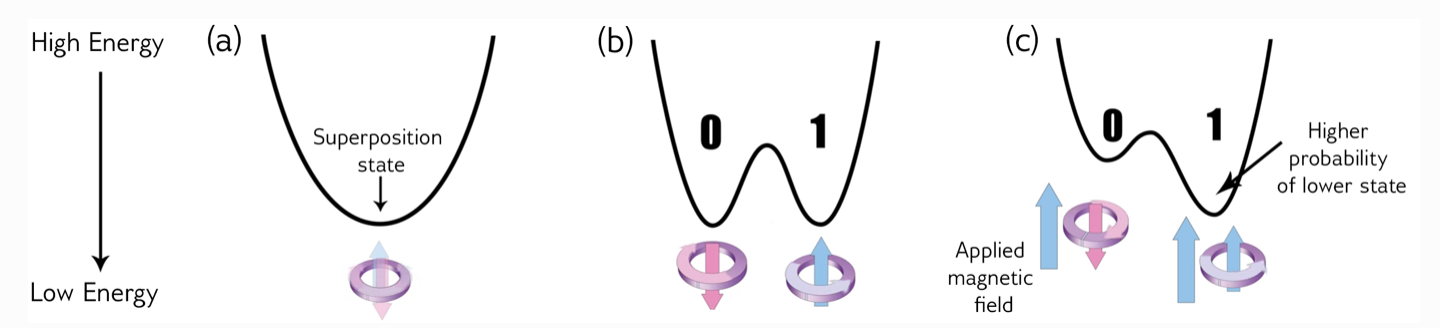
\includegraphics[width=0.6\textwidth,height=0.2\textwidth]{QA_process.png}}
\subfigure{
\label{Fig.sub.2}
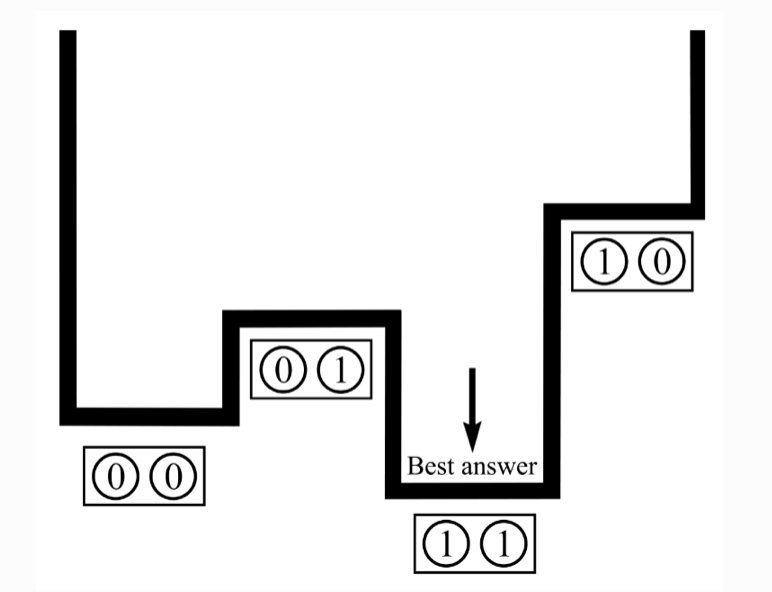
\includegraphics[width=0.25\textwidth]{QA_optimal_energy.png}}
\vspace{-0.3cm}
\caption{Energy diagram}
\label{Fig.main}
\end{figure}
%  the first: energy diagram changes over time as the quantum annealing process runs and a bias is applied.
% the second: Energy diagram showing the best answer.

\end{frame}

% ====================================================

\subsection[SQA]{Simulated Quantum Annealing}

\begin{frame}\frametitle{Simulated Quantum Annealing (SQA)}

\bit

\item A quantum-inspired algorithm that simulates the quantum tunneling phenomena.

\item The Hamiltonian of an Ising spin-glass in transverse field is
\begin{align}
\label{eq2}
    H(t)=-\sum_{(i, j)}^N J_{i j} \sigma_{i}^{z} \sigma_{j}^{z} -\Gamma(t) \sum \sigma_{i}^{x},
\end{align}
where $\sigma_{i}^{x}$ and $\sigma_{i}^{z}$ are the Pauli matrices at state $i$. % in the x and z spin bases respectively
% J_ij are interaction forces between grid neighbors.
\eit

\end{frame}

%============================================================

\subsection[Implementation]{Simulated Quantum Annealing - Implementation}
\begin{frame}\frametitle{SQA - Implementation}

\bit
\item Simulate QA via Path Integral Quantum Monte Carlo (PIQMC) \cite{santoro2002theory, suzuki1977monte} 
% approach is to employ a random sampling strategy to estimate the state space probabilities at discretized times t, involves mapping the d-dimensional quantum system into a (d+1) dimensional classical system, where we reference the extra degree of freedom as the “Trotter dimension”.

\item Each spin updates in accordance with Metropolis algorithm \cite{metropolis1953equation} with the the acceptance rate by the Eq. \eqref{eq1}.

\eit

\begin{algorithm}[H]
\algsetup{linenosize=\small}
\scriptsize
\caption{Metropolis Rule}
\begin{algorithmic}
\Function {Metropolis}{$\mathbf{s}, j, \tau$}
\State $\mathbf{s}^{\prime} \leftarrow$ configuration after the spin $s_{j}$ is flipped
\State $\Delta \leftarrow E(\mathbf{s}) - E\left(\mathbf{s}^{\prime}\right)$
\If {$\Delta$ is positive \textbf{or} $e^{\Delta / \tau}>U_{\text {random }}$ }
\State \Return{$\mathbf{s}^{\prime}$}
\Else
\State \Return{$\mathbf{s}$}
\EndFunction
\end{algorithmic}
\label{alg:metropolis}
\end{algorithm}

\end{frame}

% ==========================================

\subsection{Algorithm}
\begin{frame}\frametitle{Sketch of the Algorithm}
\begin{algorithm}[H]
\algsetup{linenosize=\small}
\scriptsize
\begin{algorithmic}[1]
\STATE $N \leftarrow$ number of spins in $H_{\text {ising }}$
\STATE $P \leftarrow$ number of Trotter slices
\STATE $T \leftarrow$ ambient temperature 
% (at end of preannealing)
\STATE $\Gamma_{\text {start }}, \Gamma_{\text {end }} \leftarrow$ starting and final magnetic field strengths
\STATE $\Gamma_{\text {step }} \leftarrow$ amount to decrease magnetic field during QA
\STATE $\mathbf{z} \leftarrow\left\{z_{0}, z_{1}, \ldots, z_{N-1}\right\}$, random initial configuration 
\\[5pt]
\STATE $\mathbf{Z} \leftarrow\left\{\mathbf{z}_{0}, \ldots, \mathbf{z}_{k}, \ldots, \mathbf{z}_{P-1}\right\}$
\\[5pt]
\FOR{$\gamma$ in $\left(\Gamma_{\text {start }}: \Gamma_{\text {end }}: \Gamma_{\text {step }}\right)$}
% $\triangleright$ simulate quantum annealing
\FOR{$Z_{i}^{k}$ in $\mathbf{Z}$}  
\STATE $\mathbf{Z} \leftarrow \operatorname{Metropolis}(\mathbf{Z}, i+k, T)$
\ENDFOR
\ENDFOR
\STATE $\mathbf{Z}_{\text{solution}} \leftarrow$ lowest energy replica amongst the $P$ Trotter slices.
\end{algorithmic}
\caption{Sketch of SQA}
\label{alg:sqa}
\end{algorithm}
\end{frame}

%============================================================
\subsection[Efficiency]{Efficient Convergence of SQA}
\begin{frame}\frametitle{Efficient Convergence of SQA}

% $$
% f(z):= \begin{cases}|z|+n^{\alpha}: & \frac{n}{4}-\frac{n^{\zeta}}{2}<|z|<\frac{n}{4}+\frac{n^{\zeta}}{2} \\ |z| & \text { o.w. }\end{cases}
% $$

% for Hamming weight with a spike
\begin{theorem}
Simulated quantum annealing based on the path-integral Monte Carlo method efficiently samples the output distribution of QA for the spike cost function under certain conditions.
\end{theorem}

\end{frame}

%============================================================

\section[Examples]{Numerical Experiments}

\subsection[Spike]{The Hamming weight with a spike}

\begin{frame}\frametitle{The Hamming weight with a spike}
Consider the cost function
$$
h(w)= \begin{cases}w, & w \neq n / 4 \\ n, & w=n / 4\end{cases}
$$
where again $w$ is the Hamming weight of $n$ bits and also $n$ is taken to be a multiple of 4 .



\bit

\item may: show spike,


\eit

\end{frame}

%=========================================================

\begin{frame}\frametitle{Result}



\end{frame}

%==============================================================

\subsection[Ising]{Ising Model with a Transverse Field}

\begin{frame}\frametitle{Ising Model with a Transverse Field}

\bit

\item Map the quantum Ising model \eqref{eq2} in a transverse field to a classical Ising model \cite{martovnak2002quantum}, 
\begin{align}
H_{q}=-\sum_{k=1}^{P}\left(\sum_{(i, j)} \frac{J_{i j}}{P} \sigma_{i, k} \sigma_{j, k}\right. \left.+J^{+} \sum_{i} \sigma_{i, k} \sigma_{i, k+1}\right),
\end{align}

where $J^{+}=T / 2 \cdot \ln \operatorname{coth}(\Gamma(t) /(P T))$.
% J+ represents the strength of couplings between replicas, and P is the number of replicas. J+ is small at the beginning of annealing and varies as the annealing proceeds. Finally, each replica will have the same spin configuration with high probability due to the sufficiently large strength of the coupling J+. Since this system converges to the thermal equilibrium, we can find the ground state with high probability by taking large enough M and small enough T.


\eit

\end{frame}

%=========================================================

\begin{frame}\frametitle{Result}



\end{frame}

%=========================================================

\section[Summary]{Summary}

\begin{frame}\frametitle{Summary}

\bit
\item SQA is exponentially faster than SA algorithm.

\vspace{0.5cm}

\item SQA can find optimal solution, while SA fails though it may be faster

\eit

\end{frame}


\section[Ref]{References}

\begin{frame}\frametitle{References}
\tiny
\bibliographystyle{unsrt}
\bibliography{references.bib}

\end{frame}

%============================================================

\frame{
\vskip30mm
\centerline{\Large\color{violet}\textsc{Thank you!}}
\vskip40mm
}

\end{document}
